\documentclass{standalone}
\usepackage{tikz}
\usepackage{ctex,siunitx,ninecolors}
\usepackage{tkz-euclide}
\usepackage{amsmath}
\usetikzlibrary{patterns, calc}
\usetikzlibrary {decorations.pathmorphing, decorations.pathreplacing, decorations.shapes}
\begin{document}
\small
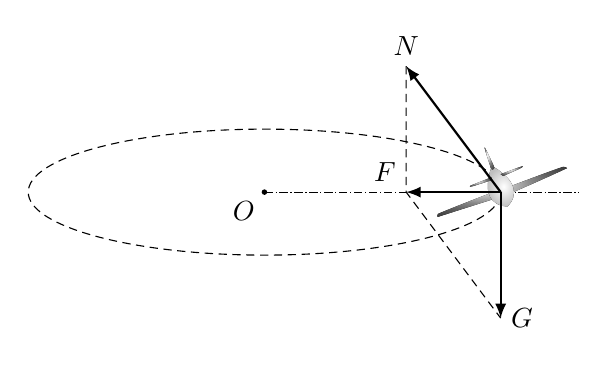
\begin{tikzpicture}[>=latex,scale=1.0]
  % \useasboundingbox(-1,-2)rectangle(8,6);
  \draw[thin,densely dashed](0,0) ellipse (3 and 0.8);
  \draw[thin,densely dashdotted](0,0)--(4,0);
  \fill(0,0)circle(1pt)node[below left]{$O$};
  \begin{scope}[xshift=1mm]
  \fill[ball color= lightgray](3.037, 0.080)..controls(3.037, 0.080)and(3.639, 0.309)..(3.698, 0.322)..controls(3.708, 0.324)and(3.749, 0.307)..(3.743, 0.304)--(3.659, 0.266)--(3.574, 0.227)--(3.489, 0.189)--(3.404, 0.151)--(3.319, 0.113)--(3.234, 0.076)--(3.148, 0.038)--(3.063, 0.001)--(2.792,-0.094)--(2.100,-0.315)..controls(2.092,-0.317)and(2.095,-0.282)..(2.103,-0.278)..controls(2.155,-0.249)and(2.759,-0.017)..(2.759,-0.017)--cycle;
  \fill[inner color=white,outer color=lightgray](2.986,-0.183)..controls(2.745,-0.170)and(2.726, 0.026)..(2.739, 0.121)..controls(2.752, 0.215)and(2.763, 0.299)..(2.796, 0.313)..controls(2.830, 0.324)and(2.893, 0.266)..(2.965, 0.203)..controls(3.036, 0.140)and(3.147,-0.022)..cycle;
  \fill[ball color= lightgray](2.932,0.205)--(3.133,0.294)..controls(3.189,0.321)and(3.197,0.334)..(3.173,0.328)..controls(3.149,0.322)and(2.899,0.228)..(2.899,0.228);
  \fill[ball color= lightgray](2.776,0.149)--(2.565,0.081)..controls(2.506,0.064)and(2.491,0.068)..(2.513,0.080)..controls(2.535,0.091)and(2.784,0.188)..(2.784,0.188);
  \fill[ball color= lightgray](2.821,0.312)..controls(2.827,0.296)and(2.803,0.290)..(2.803,0.290)..controls(2.803,0.290)and(2.783,0.278)..(2.777,0.298)..controls(2.772,0.319)and(2.689,0.564)..(2.696,0.567)..controls(2.704,0.569)and(2.814,0.328)..cycle;
  \end{scope}
  \draw[thick,->](3,0)--(3,-1.6)node[right]{$G$};
  \draw[thick,->](3,0)--(1.8,0)node[above left]{$F$};
  \draw[thick,->](3,0)--(1.8,1.6)node[above]{$N$};
  \draw[densely dashed](1.8,1.6)--(1.8,0)--(3,-1.6);
\end{tikzpicture}
\end{document}